\documentclass[11pt,letterpaper,sans]{moderncv}
\usepackage{mystd}

\begin{document}

\makecvtitle

\section{Education}
\cventry{2024 -- Today}{M1 Hadamard}
{\href{https://ens-paris-saclay.fr/}{École Normale Supérieure Paris-Saclay}}
{Gif-sur-Yvette, France}
	{}{
		Master of Science 1 in Mathematics.
		Courses are taught at \href{https://ens-paris-saclay.fr/}{\textbf{ENS Paris-Saclay}}, 
		\href{https://www.imo.universite-paris-saclay.fr/fr/}{\textbf{Orsay's Mathematical Institute}} and 
		\href{https://www.polytechnique.edu/}{\textbf{l'École Polytechnique (X)}}.
		\begin{itemize}
			\item Courses followed : Real and Functional Analysis (ENS); 
			Algebra and Galois Theory (Orsay); Advanced Probability Theory (Orsay);
			Algebraic Topology (X); Geometry (Orsay); Compact \& Lie Groups (X);
			Mathematics for Image Processing (ENS).
		\end{itemize}
	}

\cventry{2023 -- 2024}{Magistère of Mathematics}
{\href{https://ens-rennes.fr/}{École Normale Supérieure de Rennes}}
		{Rennes, France}{}{
			Result : Success at the entrance exam of the ENS Paris-Saclay (Rank 9).
			\begin{itemize}
				\item Courses followed : General Topology; Linear Algebra; Complex Analysis;
				Differential Calculus; General Group Theory; Measure Theory; Probability Theory;
				ODEs, Rings \& Arithmetics; Formal languages and computability.  
			\end{itemize}
		}
\subsection{Secondary and post-secondary}
\cventry{2021 -- 2023}{MP2I/MPI*}{Lycée Paul Valéry}{Paris 12e}{}{
	Two years in a special higher education class that prepares for competitive entrance exams
	to french Grandes Écoles. 
	"MPI" stands for "Mathematics, Physics and Computer Science". 
	As a result of these two years, I was accepted into a highly selective Grande École :
	l'École Normale Supérieure de Rennes.
}

\cventry{2019 -- 2020}{Terminale S, spécialité Mathématiques}{CNED}{}{17,77/20}{
	CNED is a French public institution that provides distance learning material. 
	I completed my last year of high school working from home, succeeded at the French baccalauréat exam, and applied to continue my studies in France.
}

\section{Work experience and internships}

\subsection{Research experience}
\cventry{May 2024 –– July 2024}{Research internship}
{\href{https://www.imo.universite-paris-saclay.fr/fr/}{Laboratoire de Mathématiques d'Orsay}}
{Orsay, France}{}{
	Magistère de mathématiques de Rennes students must spend at least six weeks in a research internship 
	at the end of the first year. \href{https://anne.vaugon.vwx.fr/}{Anne Vaugon} supervised mine at the 
	Laboratoire de Mathémaitques d'Orsay. 
	You can access my report \color{newred} 
	\href{https://perso.eleves.ens-rennes.fr/people/amar.ahmane/src/rapports/stage-l3.pdf}{here} 
	\color{black} (there's only a french version for now).\\
	During this internship, I worked on : 
	\begin{itemize}
		\item Basics of Morse Theory; 
		\item A proof of the classification of compact, connected, orientable and closed
		surfaces.\\
		\vspace{1em} 
		\begin{center}
			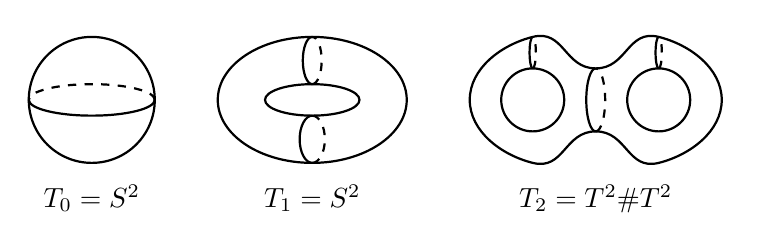
\begin{tikzpicture}[scale=.8]
    % Sphère
    \draw[thick] (0,0) circle (1cm);
    \draw[thick] (-1,0) arc (180:360:1 and .25);
    \draw[thick,dashed] (1,0) arc (0:180:1 and .25);
    \node at (0,-1.2) [below] {$T_0=\mathbb S^2$};

    % Tore 
    \draw[thick] (3.5,0) ellipse (1.5cm and 1cm);
    \draw[thick] (3.5,0) ellipse (.75cm and .25cm);
    \draw[thick] (3.5,-1) arc (270:90:.2 and .375);
    \draw[thick,dashed] (3.5,-1) arc (-90:90:.2 and .375);
    \draw[thick] (3.5,.25) arc (270:90:.15 and .375);
    \draw[thick,dashed] (3.5,.25) arc (-90:90:.15 and .375);
    \node at (3.5,-1.2) [below] {$T_1=\mathbb S^2$};

    % Quadruble tore
    \node (p1) at (6,0) {};
    \node (p2) at (7,1) {};
    \node (p3) at (8,.5) {};
    \node (p4) at (9,1) {};
    \node (p5) at (10,0) {};
    \node (p6) at (9,-1) {};
    \node (p7) at (8,-.5) {};
    \node (p8) at (7,-1) {};
    \draw[thick] (7,0) circle (.5);
    \draw[thick] (9,0) circle (.5);
    \draw[thick] (8,-.5) arc (270:90:.15 and .5);
    \draw[thick,dashed] (8,-.5) arc (-90:90:.15 and .5);
    \draw[thick] (7,.5) arc (270:90:.05 and .25);
    \draw[thick,dashed] (7,.5) arc (-90:90:.05 and .25);
    \draw[thick] (9,.5) arc (270:90:.05 and .25);
    \draw[thick,dashed] (9,.5) arc (-90:90:.05 and .25);
    \path[thick,draw] plot [smooth cycle,tension=.9] coordinates {(p1) (p2) (p3) (p4) (p5) (p6) (p7) (p8)};
    \node at (8,-1.2) [below] {$T_2=\mathbb T^2\#\mathbb T^2$};
\end{tikzpicture}
		\end{center}
	\end{itemize}
}

\subsection{Work experience}
\cventry{2024 -- Today}{Mathematics examiner (Khôlleur MPI/MPI*)}
{Lycée Paul Valéry}{Paris 12e}{}{
	I select exercises and grade CPGE students in weekly mathematics oral exams
	of 1 hour duration. 
}

\cventry{Since 2022}{Private lessons in Mathematics}{Independant}{}{}{}

\section{Computer Skills}
\cvitem{Programming}{Java, OCaml, C, Python, Javascript.}
\cvitem{Tools}{\LaTeX, git, UNIX systems.}

\section{Languages}
\cvitem{French}{Fluent}
\cvitem{English}{C1}
\cvitem{Arabic}{Fluent}

\section{Interests}
\cvitem{Academic}{Probability Theory, Functional Analysis, Optimization, Formal Languages, 
Mathematics for Data Science}
\cvitem{Other}{Video games (Minecraft, Strategy games, construction and management simulation), Tarot, 3D art...}
\end{document}